\documentclass[a4paper,11pt]{ltjsarticle}
\usepackage{amsmath, mathtools, mathbbol, amssymb, bm, cancel, fancyhdr, anyfontsize, subcaption, multirow, wrapfig, graphicx, url, enumitem, ascmac, tikz, tikz-3dplot, makeidx}
\usepackage[luatex]{hyperref}
\usepackage[most]{tcolorbox}
\usepackage{ascolorbox}
\usepackage{stackengine}
\usepackage{cleveref}

\hypersetup{
 pdfencoding=auto,
 setpagesize=false,
 bookmarksnumbered=true,
 bookmarksopen=true,
 colorlinks=true,
 linkcolor=blue,
 citecolor=blue,
 urlcolor=blue,
}

\crefname{equation}{式}{式}
\crefname{figure}{図}{図}
\crefname{table}{表}{表}

\crefname{section}{第}{第}
\creflabelformat{section}{#2#1節#3}
\crefname{subsection}{第}{第}
\creflabelformat{subsection}{#2#1節#3}

\newcommand{\crefpairconjunction}{と}
\newcommand{\crefrangeconjunction}{から}
\newcommand{\crefmiddleconjunction}{,}
\newcommand{\creflastconjunction}{,および}

\makeindex
\numberwithin{equation}{section}
\captionsetup{compatibility=false}
\usepackage[numbers]{natbib}
\usetikzlibrary{arrows, angles, quotes, cd}
\renewcommand{\cite}[1]{\textsuperscript{\citep{#1}}}
\newcommand{\idx}[1]{#1\index{#1}}

\pagestyle{fancy}
\rhead{\textbf{\thepage}}
\cfoot{}
\renewcommand{\headrulewidth}{0pt}

\title{\textbf{統計計算の基礎}}
\author{Y-teraya}
\date{\today}

\begin{document}

\pagenumbering{roman}

\maketitle

\begin{abstract}
  本資料は,統計の基礎的な計算方法をまとめたものである.
  実験計画法を主として扱い,実務で直結する内容(Excel函数など)を備忘録として記しておく.

  題材として電気学と生命化学を扱っていることには,留意していただきたい.
\end{abstract}

\tableofcontents

\vspace{12pt}

\begin{center}
  \textbf{\color{blue}青文字}をクリックすると,対応したページに遷移する.

  また本資料の著作権は,\href{https://creativecommons.org/licenses/by-nc-sa/4.0}{CC BY-NC-SA 4.0}を適応する.
\end{center}

\clearpage

\pagenumbering{arabic}

\part{数学の記法と用語}
\label{part: notations}

\section{国際単位系International System of units}
\label{sec: si}

\textbf{科学Science}の世界では,この単位系を用いて\textbf{数値と単位の組}を\textbf{物理量}Physical quantityという.
7つの\textbf{基本単位系}を組み合わせ\textbf{組立単位}にすることで,さまざまな単位を作ることができる.
組立単位を知ることによって,求めたい単位に変える\textbf{単位換算}Unit conversionを行うことができるようになる.

\subsection{基本単位系Basic units}
\label{sec: basic units}

基本単位は次の7つである.

\begin{table}[hbtp]
  \caption{基本単位系}
  \label{tab: basic units}
  \centering
  \begin{tabular}{rll}
    \hline
    データの種類 & 英語 & 単位 \\
    \hline
    時間 & {\color{cyan}$t$}ime & [s] \\
    距離 & {\color{cyan}$r$}oute & [m] \\
    電流 & {\color{cyan}$I$}ntensity of current & [A] \\
    質量 & {\color{cyan}$m$}ass & [g] \\
    絶対温度 & {\color{cyan}$T$}emperture & [K] \\
    物質量 & {\color{cyan}$n$}umber & [mol] \\
    光度 & Luminous {\color{cyan}$I$}ntensity & [cd] \\
    \hline
  \end{tabular}
\end{table}

\begin{ascolorbox4}[基本単位系の定義\cite{units-1}]{余談}
\label{col: basic def}

  \hspace{5pt}

   基本単位系には,\textbf{一義性}\footnote{ただ1つに定まる性質のこと.}と\textbf{普遍性}\footnote{広く全ての場合にあてはめることができる性質のこと.}を持った基準が必要であり世界共通のものである.
  その\textbf{厳密な定義}を紹介する.

  \subsubsection{時間の定義\cite{units-2}}

   原子や分子には,固有の振動数の光や電波を吸収し放射する性質がある.その性質を利用して,セシウム原子のマイクロ波の振動$\Delta \nu_{\mathrm{Cs}}$を,$9,192,631,770$回数えたときを1秒と定義した.
  [Hz]\footnote{ヘルツは,\textbf{回数}を示す単位である.}は\textbf{単位時間あたりの振動数}のことであり,[/s]と同じ意味である.

  \subsubsection{距離の定義}

   真空中の光の速さ$c$を$299,792,458$ [m/s]と定めることによって定義した.

  \subsubsection{電流の定義\cite{units-5}}

   かつては,真空中に1\ [m]間隔で平行に置いた無限に長い2本の導体がそれぞれを流れ,これらの導体の長さ1\ [m]につき$2 \times 10^{-7}$\ [N]の力を及ぼし合う一定の電流を1\ [A]としていた.
  ただし,電流の単位を力として定義している.これは\textbf{電流は素粒子の流れ}であるという本質が分かっていなかったためである.そのため,2019 年に改定された.

   新たに電気素量$e$\footnote{ファラデー定数(電子1 [mol]が持つ電気量の値のこと)を$F$,アボガドロ定数を$N_A$とすると,$e=\tfrac{F}{N_A}$でも求められる.}を$1.602,176,634 \times 10^{−19}$ [C]と定めることによって定義した.
  [C]は\textbf{単位時間あたりの電気量}のことであり,$\mathrm{[A \cdot s]}$と同じ意味である.

  \subsubsection{質量の定義\cite{units-3}}

   かつては,国際キログラム原器(白金とイリジウムの合金で出来た円柱)の質量を1\ [kg]としていた.
  ただし,経年劣化により一義性に欠けるため,電流と同様に2019年に改定された.
  
   物体の静止質量を$m$,光子の周波数を$\nu$,プランク定数を$\hslash$とすると,
  アインシュタインの相対性理論によれば次である.

  \begin{equation}
    E = mc^2 = \hslash \nu \label{eq: einstein}
  \end{equation}

   ここでプランク定数$\hslash$を$6.626,070,15 \times 10^{−34}\ \mathrm{[J \cdot s]}$と定義することで,
  周波数$\nu$\ [Hz]の光子のエネルギー$E$と等価な質量が$m$\ [kg]である.

  \subsubsection{絶対温度の定義\cite{units-4}}

   かつては,氷と水,水蒸気が共存する温度$0.01 ^\circ \mathrm{C}$の約273分の1を1\ [K]としていた.
  ただし,「水」という物質に依存しており,かつ三重点の実現可能性が低いため電流と同様に2019年に改定された.

   理想気体の場合,個々の分子は他の分子と衝突するとき以外は自由に動く.
  1個の単原子の平均の運動エネルギーは,質量を$m$,2乗平均速度を$\overline{v^2}$,ボルツマン定数$k$,絶対温度$T$とすると次である.

\begin{subequations}

  \begin{equation}
    \frac{1}{2} m \overline{v^2} = \frac{3}{2} kT \label{eq: boltzmann-1}
  \end{equation}

   一方で,理想気体の分子$nN_A$個\footnote{$N_A$はアボガドロ定数であり,ボルツマン定数$k$と乗算することで気体定数$R$となる.}を体積$V$の容器に入れた場合,その圧力$p$は,質量$m$と2乗平均速度$\overline{v^2}$とすると次である.

  \begin{equation}
    p = \frac{1}{3} \frac{nN_Am}{V} \overline{v^2} \label{eq: boltzmann-2}
  \end{equation}

   \cref{eq: boltzmann-1,eq: boltzmann-2}より,次の理想気体の状態方程式が得られる.

  \begin{equation}
    p(T)V = nN_AkT \label{eq: air}
  \end{equation}

\end{subequations}

   エネルギーは$[\mathrm{J}] = [\mathrm{kg \cdot m^2/s^2}]$で表される.
  ここでボルツマン定数$k$を$1.380, 649 \times 10^{−23}$\ [J/K]と定義することで,単位の大きさを定めることと同じになる.

  \subsubsection{物質量の定義\cite{units-6}}

   原子1粒同士を比較しても,非常に小さいため明確に重さの違いは分からない.しかし,何万,何億の粒を集めて比較すると,違いが分かるようになる.
  かつては,炭素原子を基準として12\ [g]になるために必要な数である$6.022 \times 10^{23}$個(アボカドロ数)を1\ [mol]としていた.ただし,絶対温度の同じように今回は「炭素」依存での定義であり普遍性に欠ける.そのため,電流と同様に2019年に改定された.

   ここでアボガドロ定数$N_A$を$6.022,140,76 \times 10^{23}$\ [/mol]と定義することで,単位の大きさを定めた.
  簡単にいれば,原子や分子の粒を$N_A$個のことを1\ [mol]と置いた.この考えは,12個を1ダースと置くのと同じである.

  \subsubsection{光度の定義}

   特定の周波数$540 \times 10^{12}$\ [Hz]の緑色の光を出す特定の方向に,放射強度$K_{\mathrm{cd}}$が683 [lm/W]である点光源の光度を,1\ [cd]と定義した.

\end{ascolorbox4}

\clearpage

\subsection{接頭辞Prefix}
\label{sec: prefix}

接頭辞とは,基本単位系よりも\textbf{大きい・小さいことを表す指標}のことである.
Si接尾辞では$\times 10^{\pm 30}$まで定まっているが,よく使われる$\times 10^{\pm 12}$までを紹介する.

\begin{table}[htbp]
  \caption{Si接頭辞}
  \label{tab: prefix}
  \centering
  \begin{tabular}{cccccc}
    \hline
    ($+$)接頭辞 & 英語 & 指数乗 & ($-$)接頭辞 & 英語 & 指数乗 \\
    \hline
    T & {\color{cyan}T}era & $\times 10^{12}$ & p & {\color{cyan}p}ico & $\times 10^{-12}$ \\
    G & {\color{cyan}G}iga & $\times 10^{9}$ & n & {\color{cyan}n}ano & $\times 10^{-9}$ \\
    M & {\color{cyan}M}ega & $\times 10^{6}$ & $\mu$ & micro & $\times 10^{-6}$ \\
    k & {\color{cyan}k}ilo & $\times 10^{3}$ & m & {\color{cyan}m}illi & $\times 10^{-3}$ \\
    h & {\color{cyan}h}ecto & $\times 10^{2}$ & c & {\color{cyan}c}enti & $\times 10^{-2}$ \\
    da & {\color{cyan}d}ec{\color{cyan}a} & $\times 10^{1}$ & d & {\color{cyan}d}eci & $\times 10^{-1}$ \\
    \hline
  \end{tabular}
\end{table}

\subsection{単位換算Unit conversion}
\label{sec: convertion}

単位は,\textbf{定義に基づいて}組み立てることで新しい単位ができる.
基本的には,\textbf{同じ意味を持つもの同士を分母と分子に置き},{\color{cyan}\textbf{約分する}}ことで求めたい単位へと変える.
\cref{eq: uc-1}は,「\textbf{1日は何秒か?}」を求めたものである.恐らく,一度は計算したことがあるだろう.

\begin{equation}
  1\ [\mathrm{day}] = 1\ \cancel{[\mathrm{day}]} \times \frac{24\ \cancel{[\mathrm{hr}]}}{1\ \cancel{[\mathrm{day}]}} \times \frac{60\ \cancel{[\mathrm{min}]}}{1\ \cancel{[\mathrm{hr}]}} \times \frac{60\ [\mathrm{sec}]}{1\ \cancel{[\mathrm{min}]}} = 86,400\ [\mathrm{sec}] \label{eq: uc-1}
\end{equation}

単位換算を行う上で押さえるポイントは,最初の単位と\textbf{求めたい単位に注目し}
定義として\textbf{どの物理量同士が等しいか}考え約分する必要がある.
今回の場合,1\ [day] と 24\ [hr]は定義より等しいので,分母と分子に置くことで理論上約分でき1と同じ意味となる.

次に,\cref{sec: prefix}の接頭辞を用いた単位換算を扱う.一例として,[mL]を[L]に変える場合を考える.

\begin{equation}
  1,000\ [\mathrm{{\color{cyan}m}L}] = 1,000 \times {\color{cyan}10^{-3}}\ [\mathrm{L}] = 1\ [\mathrm{L}] \label{eq: uc-2}
\end{equation}

[mL]の{\color{cyan}m}は,\cref{tab: prefix}を参照すると指数乗は{\color{cyan}$10^{-3}$}である.
そのため,まず\textbf{接頭辞を指数乗に変える}.そのあと,指数乗を掛けることで単位を換算できる.

\clearpage

その他,戸惑いやすいが変換できるものを紹介する.

\begin{table}[htbp]
  \caption{単位変換}
  \label{tab: unit}
  \centering
  \begin{tabular}{rlrl}
    \hline
    \multicolumn{2}{c}{物理学} & \multicolumn{2}{c}{生命化学} \\
    \hline
    ニュートン & 1\ [N] := 1\ [kg \cdot m/s$^2$] & 体積と質量 & 1\ [cc] = 1\ [mL] = 1\ [g] \\
    角度 & 1\ [deg] := $\tfrac{\pi}{180}$\ [rad] & 体積と体積 & 1\ [L] := 1\ [dm$^3$] = 0.001\ [m$^3$] \\
    パスカル & 1\ [Pa] := 1\ [kg/m \cdot s$^2$] & モル濃度 & 1\ [M] := 1\ [mol/L] \\
    ジュール & 1\ [J] := 1\ [N \cdot m] & 水素イオン係数 & $\mathrm{pH} := - \log[\mathrm{H}^+]$ \\
    ワット & 1\ [W] := 1\ [J/s] & 温度 & 1\ $[^\circ \mathrm{C}] := -273.15$\ [K] \\
    クーロン & 1\ [C] := 1\ [A \cdot s] \\
    ボルト & 1\ [V] := 1\ [W/A] = 1\ [J/C] \\
    ヘルツ & 1\ [Hz] := 1\ [/s] \\
    \hline
  \end{tabular}
\end{table}

詳しく調べたい場合は,\href{https://www.dainippon-tosho.co.jp/unit/list}{\textbf{大日本図書 いろいろな単位}}が分かりやすいので紹介しておく.

\subsection{ギリシャ文字Greek alphabet}

よく数式の記号でギリシャ文字が用いられるので,知っていると役に立つだろう.

\begin{table}[htbp]
  \caption{ギリシャ文字}
  \label{tab: greek}
  \centering
  \begin{tabular}{rcccrccc}
    \hline
    読み方 &  & 大文字 & 小文字 & 読み方 &  & 大文字 & 小文字 \\
    \hline
    alpha & アルファ & A & \alpha & beta & ベータ & B & \beta \\
    gamma & ガンマ & \Gamma & \gamma & delta & デルタ & \Delta & \delta \\
    epsilon & イプシロン & E & \varepsilon, \epsilon & zeta & ゼータ & Z & \zeta \\
    eta & イータ & H & \eta & theta & シータ & \Theta & \theta, \vartheta \\
    iota & イオタ & I & \iota & kappa & カッパ & K & \kappa \\
    lambda & ラムダ & \Lambda &\lambda & mu & ミュー & M & \mu \\
    nu & ニュー & N & \nu & omicron & オミクロン & O & $o$ \\
    xi & クシー, グザイ & \Xi & \xi & pi & パイ & \Pi & \pi, \varpi \\
    pho & ロー & P & \rho, \varrho & sigma & シグマ & \Sigma & \sigma, \varsigma \\
    tau & タウ & T & \tau & upsilon & ウプシロン & \Upsilon & \upsilon \\
    phi & ファイ & \Phi & \phi, \varphi & chi & カイ & X & \chi \\
    psi & プサイ & \Psi & \psi & omega & オメガ & \Omega & \omega \\
    \hline
  \end{tabular}
\end{table}

\clearpage

\part{初歩的な計算}
\label{part: calculate}

\section{指数Exponent}
\label{sec: exponent}

\subsection{累乗Repeat multiplication}
\label{sec: repeat}

任意の\footnote{「すべての」,「どんな」,「どれを選んでも」と同じ意味である.}$a$を$n$回掛けたものを$a$の$n$乗といい$a^n$\footnote{指数が複雑な場合,$a\exp(n)$と表記される場合もある.}と書く.$a$を\textbf{底}Base,$n$を\textbf{指数}Exponentという.
特に,指数が正の整数($n > 0$)のとき\textbf{累乗}Repeat multiplicationといい,それ以外の場合は,\textbf{べき乗}Powerという.

指数法則Exponential lawsは,定義より自明\footnote{一般に法則として紹介されていることが多いので,本資料では法則として扱う.また一般に法則とは,経験則から導かれた証明できない事象のことを指す.}である.
底を$a$,指数を$m, n$としたとき,次の2法則が成立する.

\begin{equation}
  a^m \times a^n = \underbrace{a \times a \times a \times \cdots \times a}_\text{\bm{m}\textbf{\normalsize 個}} \cdot \underbrace{a \times a \times \cdots \times a}_\text{\bm{n}\textbf{\normalsize 個}} = a^{m+n} \label{eq: rpt-1}
\end{equation}

これは単純.$a$を$m$回掛けたものと$a$を$n$回掛けたものを全て乗算したら,$a$を$m+n$回掛けたものと同じになる.

\def\tmp{%
  \begin{matrix}
  a & \times & a & \times & \cdots & \times & a \\
  a & \times & a & \times & \cdots & \times & a \\
  \vdots &  & \vdots &  & \ddots &  & \vdots \\
  a & \times & a & \times & \cdots & \times & a \\
  \end{matrix}
}
\begin{equation}
  \big(a^m\big)^n =\ 
  \stackMath\def\stackalignment{r}%
  \stackunder%
  {\text{\bm{n}\textbf{\normalsize 個}}\left\{\tmp\right.}%
  {\underbrace{\phantom{\smash{\tmp\mkern 0mu}}}_\text{\bm{m}\textbf{\normalsize 個}}\mkern 0mu}%
  \ =a^{m \times n} \label{eq: rpt-2}
\end{equation}


少し捉えにくいかもしれない.\cref{eq: rpt-2}のように,$a$を$m$回掛けたものを縦に$n$個並べる.
それは$a$を$m \times n$に並べた長方形となり,$m \times n$回乗算したものと同じだと分かる.
このように,視覚的に理解できるだろう.

\cref{eq: rpt-1,eq: rpt-2}は特に暗記しなくても,\textbf{累乗がどういうものだったか?}を考えれば簡単に分かる.

\subsection{0乗とマイナス乗}

\cref{eq: rpt-1}が正しいと仮定すると,0乗とマイナス乗を定義できる.まず,\cref{eq: rpt-1}を$n=0$とすると次である.

\begin{subequations}

\begin{equation}
  a^m \times a^0 = a^{m+0} = a^m \label{eq: zrp-1}
\end{equation}

$a^m$に$a^0$を乗算しても\textbf{変化しない}.その数は,{\color{cyan}\textbf{1}}なので次と定義される.

\begin{equation}
  a^0 := 1 \label{eq: zrp-2}
\end{equation}

\end{subequations}

\cref{eq: zrp-2}が正しいと仮定し,\cref{eq: rpt-1}を$n=-m$とすると次である.

\begin{subequations}

\begin{equation}
  a^m \times a^{-m} = a^{m-m} = a^0 = 1 \label{eq: mnp-1}
\end{equation}

$a^m$に$a^0$を乗算すると\textbf{1になる}.その数は,{\color{cyan}\textbf{逆数}}
\footnote{任意の数に\textbf{乗算すると1になる数}のこと.}なので次と定義される.

\begin{equation}
  a^{-m} := \frac{1}{a^m} \label{eq: mnp-2}
\end{equation}

\end{subequations}

\subsection{累乗根Radical root}
\label{sec: radical}

$n$乗すると任意の数$a$になる数のことを累乗根Radical rootといい$\sqrt[n]{a}$と書く.$n$乗を強調して,\textbf{$\bm{n}$乗根}ともいう.
また,$n=2$のとき,\textbf{平方根}Square rootといい$\sqrt{a}$と書き,ルートの左肩の2は省略できる.
ただし,ルートで表記するのは見ずらくなるので指数で表現したい.指数方程式を解くことで累乗根を指数で定義できる.
$a$を\textbf{底},$n$を\textbf{指数}と次である.

\begin{subequations}

\begin{equation}
  \sqrt[n]{a} = a^x \label{eq: ipr-1}
\end{equation}

辺々\footnote{両辺と同じ意味.左辺(左側の式)と右辺(右側の式)の両方の式という意味である.}$n$乗すると,次である.

\begin{equation}
  \big(\sqrt[n]{a}\big)^n = \big(a^x\big)^n \label{eq: ipr-2}
\end{equation}

左辺はルートが外れ,指数で表現される.また,分かりやすいように1乗として書くと次である.

\begin{equation}
  a^1 = a^{nx} \label{eq: ipr-3}
\end{equation}

底が同じ方程式\footnote{等号で結ばれた式のこと.}は,指数も同じである\footnote{これが指数方程式の基本的な考え方である.}.
指数だけ取り出して等式にすると,次である.

\begin{equation}
  1 = nx \label{eq: ipr-4}
\end{equation}

$x$について解き,$n$乗根を指数で表すと次で定義される.

\begin{equation}
  \sqrt[n]{a} := a^{\tfrac{1}{n}} \label{eq: ipr-5}
\end{equation}

\end{subequations}

\clearpage

\part{統計のデータ}
\label{part: statistics}

\section{\idx{代表値}\idx{Average}}
\label{sec: average}

データ全体を分布中心のデータ1つで表したものを\idx{代表値}という.
主に3つの値のことを指し,\idx{平均値}\idx{Mean},\idx{中央値}\idx{Median},\idx{最頻値}\idx{Mode}である.
ただし,これらの値がデータの代表ではない可能性もあるため,
扱うときには必ずデータの代表として機能しているのか確認する必要がある\cite{ave-1,ave-2}.

\subsection{\idx{平均値}\idx{Mean}}
\label{sec: mean}

主に\idx{算術平均}のことを指す.全データを合計し,データの数で割ることで求められる.
\idx{平均値}を $\overline{x}$\footnote{$\mu$と置くこともある.},データ数を$n$,各データを$x_k$とすると,次と定義\footnote{$:=$は\textbf{左辺を右辺と定義する}と示す記号である.}する
\footnote{$\sum$の計算は,基本的に$1 \leq k \leq n\ (k \in \bm{Z})$の範囲内での\textbf{総和}を示す記号である.$\sum$の下に書いてある数字から,上に書いてある数字までを\textbf{カウントアップして足したもの}である.}.

\begin{equation}
  \overline{x} := \frac{1}{n} \sum_{k=1}^n x_k = \frac{x_1 + x_2 + \cdots + x_n}{k} \label{eq: ave-1}
\end{equation}

\begin{ascolorbox10}{平均値\ 概要}

  \begin{description}
    \item[メリット\cite{ave-3}] 全てのデータを考慮できる.
    \item[デメリット] \idx{外れ値}に弱い.
    \item[エクセル] =AVERAGE(Cell\textsubscript{1}:\ Cell\textsubscript{2})
  \end{description}

\end{ascolorbox10}

\begin{ascolorbox4}[平均にもいろんな種類がある!\cite{ave-4}]{余談}
\label{col: average}

  \hspace{5pt}

   上記では,算術平均(相加平均)を取り扱った.一般に平均と言われればこの算術平均だと思えばよい.
  ただ,他にも場合によっては使える平均があるので紹介する.

  \subsubsection{幾何平均(相乗平均)}

   算術平均は足し算においての平均であったが,これは掛け算においての平均である.
  \idx{平均値}を $G$,データ数を$n$,各データを$x_k$とすると,次である
  \footnote{$\prod$の計算は$\sum$の足し算を\textbf{掛け算に変えた}ものである,基本的に$1 \leq k \leq n\ (k \in \bm{Z})$の範囲内での\textbf{総積}を示す記号である.$\prod$の下に書いてある数字から,上に書いてある数字までを\textbf{カウントアップして掛けたもの}である.}.

  \begin{equation}
    G := \left(\prod_{k=1}^n x_k\right)^{\tfrac{1}{n}} = \sqrt[n]{x_1 \times x_2 \times \cdots \times x_n} \label{eq: ave-2}
  \end{equation}

   主に,成長率や増加率など\textbf{比率や割合で変化する数の平均}を算出したいときに用いる.

  \subsubsection{調和平均}

   調和平均は,一度逆数にしたデータの算術平均のことである.
  \idx{平均値}を $H$,データ数を$n$,各データを$x_k$とすると,次である.

  \begin{equation}
    H^{-1} := \frac{1}{n} \left(\sum_{k=1}^n \frac{1}{x_k}\right) = \frac{\frac{1}{x_1} + \frac{1}{x_2} + \cdots + \frac{1}{x_n}}{n} \label{eq: ave-3}
  \end{equation}

   主に,平均速度や並列接続時の抵抗,直列接続時のコンデンサなど\textbf{比率で表わされる数の平均}を算出したいときに用いる.

\end{ascolorbox4}

\subsection{\idx{中央値}\idx{Median}}
\label{sec: median}

データを\textbf{大きさの順に}並べた際の,真ん中の値を指す.例えば,データの集合$A$を次と設定する.

\begin{equation}
  A = \{x_k|1 \leq k \leq 5\} \label{eq: med-1}
\end{equation}

数列$x_k$が昇べきの順に並んでいるとすると,集合$A$の\idx{中央値}は$x_3$である.

\begin{ascolorbox10}{中央値\ 概要}

  \begin{description}
    \item[メリット\cite{ave-3}] \idx{外れ値}に強い.
    \item[デメリット] 全てのデータを十分に考慮に入れることができない.
    \item[エクセル] =MEDIAN(Cell\textsubscript{1}:\ Cell\textsubscript{2})
  \end{description}

\end{ascolorbox10}

\subsection{\idx{最頻値}\idx{Mode}}
\label{sec: mode}

データの集合内で,同じデータが存在する場合がある.その同じデータが最も出現する値を指す.例えば,集合$A$,\cref{eq: med-1}に次と設定する.

\begin{equation}
  x_2 = x_3 \label{eq: mod-1}
\end{equation}

このとき,集合$A$の\idx{最頻値}は$x_2$,$x_3$である.

\begin{ascolorbox10}{最頻値\ 概要}

  \begin{description}
    \item[メリット\cite{ave-3}] \idx{外れ値}に強い.
    \item[デメリット] 1つに決まらないことがある.また,サンプルサイズが少ないと使えない.
    \item[エクセル] =MODE.SNGL(Cell\textsubscript{1}:\ Cell\textsubscript{2})
  \end{description}

\end{ascolorbox10}

\subsection{\idx{最大値}\idx{Maximum}・\idx{最小値}\idx{Minimum}}
\label{sec: max-min}

データの集合内で,一番大きい値を\idx{最大値},小さい値を\idx{最小値}という.例えば,集合$A$,\cref{eq: med-1}を基にして考える.
このとき,\idx{最大値}は$x_5$,\idx{最小値}は$x_1$である.

\begin{ascolorbox10}{最大値・最小値\ 概要}

  \begin{description}
    \item[エクセル(最大値)] =MAX(Cell\textsubscript{1}:\ Cell\textsubscript{2})
    \item[エクセル(最小値)] =MIN(Cell\textsubscript{1}:\ Cell\textsubscript{2})
  \end{description}

\end{ascolorbox10}

\section{\idx{散布度}\idx{Dispersion}}
\label{sec: dispersion}

\subsection{\idx{分散}\idx{Variance}・\idx{標準偏差}\idx{Standard deviation}}
\label{sec: variance}

各データと\textbf{平均との差}の平均である.一般にデータの\textbf{バラつき}を表す.\idx{分散}を$s^2$\footnote{$\sigma^2$と置くこともある.},データ数を$n$,各データを$x_k$とすると,次である.

\begin{equation}
  s^2 := \frac{1}{n} \sum_{k=1}^n (x_k - \overline{x})^2= \dfrac{(x_1 - \overline{x})^2 + (x_2 - \overline{x})^2 + \cdots + (x_n - \overline{x})^2}{n} \label{eq: var-1}
\end{equation}

\idx{標準偏差}はこの2乗を外したもののことである.すなわち,\idx{分散}$s^2$をルート$\sqrt{\quad}$に入れたものである.そのため,\idx{標準偏差}を$s$\footnote{$\sigma$と置くこともある.}とすると次である.

\begin{equation}
  s := \sqrt{\frac{1}{n} \sum_{k=1}^n (x_k - \overline{x})^2} \label{eq: sdv-1}
\end{equation}

\begin{ascolorbox4}[なぜ2乗した誤差を考えるのか?\cite{var-1}]{余談}
\label{col: error}

  \hspace{5pt}

   平均との差であれば,絶対値を用いれば良いと考えられる.絶対値で計算する平均偏差と呼ばれるものを紹介する.平均偏差は次で求められる.

  \begin{equation}
    MAE = \frac{1}{n} \sum_{k=1}^n |x_k - \overline{x}| \label{eq: err-1}
  \end{equation}

   ただし,これは数学的に扱いにくい.次に3点挙げる.

  \begin{enumerate}
    \item 絶対値は函数として微分可能でなく扱いづらい.
    \item 場合分けが必要になることがある.
    \item $\displaystyle{\overline{x} \ne \arg \min_{\overline{x}} \sum_{k=1}^n |x_k - \overline{x}|}$である.
  \end{enumerate}

   特に3つ目が問題であるが,説明は参考文献の記事に譲る.

\end{ascolorbox4}

\subsection{\idx{範囲}\idx{Range}}
\label{sec: range}

単に\idx{最大値}と\idx{最小値}の差である.例えば,集合$A$,\cref{eq: med-1}を基にして考える.
このとき,\idx{範囲}は$x_5 - x_1$である.

\clearpage

\part{データのイメージ}
\label{part: deta}

\section{スカラーScalarとベクトルVector}
\label{sec: sca-vec}

スカラーは\textbf{1つの数}であり,ベクトルは\textbf{2つ以上の数を束ねたもの}である.
スカラーはそのまま,ベクトルは\textbf{太字}$\bm{x}$または\textbf{2重文字}$\mathbb{x}$(文字に余計な線を1つ入れるだけ)で表現する
\footnote{高校までは文字の上に矢印$\vec{x}$を描いてベクトルを表現した.ただし,\textbf{見づらく}なりやすいという欠点があるため,大学以降ではあまり使われない.}.
よく,スカラーは大きさ\textbf{だけ}持つ量で,ベクトルは大きさと\textbf{向きも}持つ量と理解している人も多い.{\color{cyan}\textbf{それは何故か?}}

\begin{figure}[htbp]
\centering
\begin{minipage}[b]{0.49\columnwidth}
  \centering
  \begin{equation}
    A = 2 \label{eq: sca-1}
  \end{equation}
  \caption{スカラー量}
  \label{eq: sca-quantity}
\end{minipage}
\begin{minipage}[b]{0.49\columnwidth}
  \centering
  \begin{equation}
    \bm{B} = (2 \qquad 1 \qquad 3) \label{eq: vec-1}
  \end{equation}
  \caption{ベクトル量}
  \label{eq: vec-quantity}
\end{minipage}
\end{figure}

スカラーのイメージは,\textbf{1次元}である.すなわち,$x$軸だけの数直線を考えると単なる\textbf{大きさ}にすぎない.
次にベクトルのイメージは,\textbf{2次元}や\textbf{3次元}である.$x$軸だけでは,大きさしか表せなかったのに対し,
数を束にすることで\textbf{2つ目以降の数によって方向が決まる}.

\begin{figure}[htbp]
\centering
\begin{minipage}[b]{0.49\columnwidth}
  \centering
  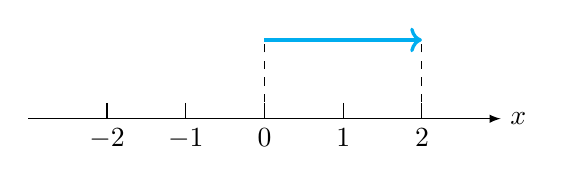
\begin{tikzpicture}
    \draw[-latex] (-3,0) -- (3,0) node[right]{$x$};
    \foreach \x in {-2,...,2} \draw (\x,0.2)--(\x,0) node[below] {$\x$};
    \draw[->, very thick, cyan] (0,1) -- (2,1);
    \draw[dashed] (0,0) -- (0,1);
    \draw[dashed] (2,0) -- (2,1);
  \end{tikzpicture}
  \caption{スカラーのイメージ}
  \label{fig: sca-image}
\end{minipage}
\begin{minipage}[b]{0.49\columnwidth}
    \centering
    \begin{tikzpicture}
      \draw[-latex] (0,0,0) -- (4,0,0) node[right]{$x$};
      \foreach \x in {1,...,3} \draw (\x,0.2,0)--(\x,0,0) node[below] {$\x$};
      \draw[-latex] (0,0,0) -- (0,4,0) node[above]{$z$};
      \foreach \z in {0,...,3} \draw (0.2,\z,0)--(0,\z,0) node[left] {$\z$};
      \draw[-latex] (0,0,0) -- (0,0,4) node[below]{$y$};
      \foreach \y in {1,...,3} \draw (0.2,0,\y)--(0,0,\y) node[above left] {$\y$};
      \draw[->, very thick, cyan] (0,0,0) -- (2,3,1);
      \draw[dashed] (2,0,0) -- (2,0,1) -- (0,0,1);
      \draw[dashed] (2,3,0) -- (2,3,1) -- (0,3,1) -- (0,3,0) --cycle;
      \draw[dashed] (2,0,0) -- (2,0,1) -- (0,0,1);
      \draw[dashed] (2,0,0) -- (2,3,0);
      \draw[dashed] (2,0,1) -- (2,3,1);
      \draw[dashed] (0,0,1) -- (0,3,1);
    \end{tikzpicture}
    \caption{ベクトルのイメージ}
    \label{fig: vec-image}
\end{minipage}
\end{figure}

簡単に説明すると,スカラーは\textbf{1つの}数であり,ベクトルは\textbf{数と数の組}\footnote{厳密には,\textbf{線形空間の元}である.線形空間の元として考えると,多項式もベクトル,函数もベクトル,微分方程式の解もベクトルとして捉えられる.これらのように,この世界にはベクトルでありふれている!}である.
ベクトルは方向を表すことから,基本的に\textbf{矢印}で表現することが多い.そのとき大きさは,矢印の\textbf{長さ}で表す.

\subsection{ベクトルの加減法}
\label{sec: vec-cal}

スカラーはそのまま加減乗除できるが,ベクトルはそう上手くいかない.ベクトルの乗法には\textbf{内積}と\textbf{外積}の2種類あり,除法はできない.
分かりやすい加減法から説明する.

言葉で説明すると,矢印の終点ともう一方の矢印の始点を合わせ,1つの折れ線矢印と見なして始点と終点を線で結ぶ.減法の場合は,矢印を逆にしてから足す.
矢印が逆のベクトルを\textbf{逆ベクトル}という.

\hspace{0pt}

\begin{figure}[htbp]
\centering
\begin{minipage}[b]{0.32\columnwidth}
  \centering
  \begin{tikzpicture}
    \draw [-latex,thick] (0,0)--(1,2);
    \node [above left] at ($(0,0)!0.5!(1,2)$) {$\bm{b}$};
    \draw [-latex,thick] (1,0)--(4,0);
    \node [below] at ($(1,0)!0.5!(4,0)$) {$\bm{a}$};
  \end{tikzpicture}
  \caption{$\bm{a}$と$\bm{b}$}
  \label{fig: vec-a, b}
\end{minipage}
\begin{minipage}[b]{0.32\columnwidth}
  \centering
  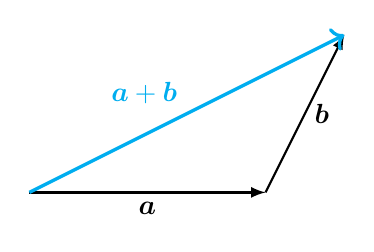
\begin{tikzpicture}
    \draw [-latex,thick] (3,0)--(4,2);
    \node [right] at ($(3,0)!0.5!(4,2)$) {$\bm{b}$};
    \draw [-latex,thick] (0,0)--(3,0);
    \node [below] at ($(0,0)!0.5!(3,0)$) {$\bm{a}$};
    \draw [->,very thick,cyan] (0,0)--(4,2);
    \node [above left,cyan] at ($(0,0)!0.5!(4,2)$) {$\bm{a}+\bm{b}$};
  \end{tikzpicture}
  \caption{三角形を作る方法}
  \label{fig: triangle}
\end{minipage}
\begin{minipage}[b]{0.32\columnwidth}
  \centering
  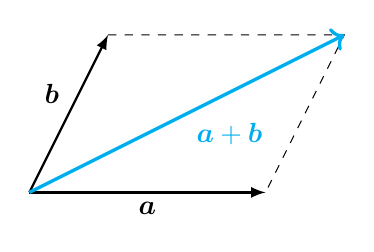
\begin{tikzpicture}
    \draw [-latex,thick] (0,0)--(1,2);
    \node [above left] at ($(0,0)!0.5!(1,2)$) {$\bm{b}$};
    \draw [-latex,thick] (0,0)--(3,0);
    \node [below] at ($(0,0)!0.5!(3,0)$) {$\bm{a}$};
    \draw [dashed] (1,2)--(4,2)--(3,0);
    \draw [->,very thick,cyan] (0,0)--(4,2);
    \node [below right,cyan] at ($(0,0)!0.5!(4,2)$) {$\bm{a}+\bm{b}$};
  \end{tikzpicture}
  \caption{平行四辺形を作る方法}
  \label{fig: parallelogram}
\end{minipage}
\end{figure}

\subsection{単位ベクトル}
\label{sec: vec-unit}

ユークリッド空間(実数を$n$個並べた全体の集合)において,3つの直交座標をそれぞれ$x$軸,$y$軸,$z$軸とする.
そのなかで\textbf{大きさを「1」に仕立てた}ベクトルを単位ベクトル\footnote{単位**は基本的に,**の大きさを「1」に仕立てたもののことである.}という.

また,$x$軸と平行な単位ベクトルを$\bm{i}$,$y$軸と平行な単位ベクトルを$\bm{j}$,$z$軸と平行な単位ベクトルを$\bm{k}$とする.

\subsection{ベクトルの成分表示Component form}
\label{sec: component}

単位ベクトルと係数倍を用いて,一般にベクトルを次のような式で表せる.

\begin{equation}
  \bm{a}=A \bm{i}+B \bm{j}+C \bm{k} \label{eq: cpf-1}
\end{equation}

また,係数を座標のように表して,

\begin{equation}
  \bm{a}=(A \quad B \quad C) \label{eq: cpf-2}
\end{equation}

とも表せる.

\clearpage

\pagenumbering{alph}

\lhead{}
\bibliographystyle{plain}
\bibliography{ref.bib}
\nocite{*}

\printindex

\end{document}